\section{Instrumentos y elementos empleados}

Para el desarrollo de la experiencia, se utilizaron los siguientes instrumentos de medición y fuentes de energía, los cuales pueden observarse en la Figura \ref{fig:fotos_laboratorio}:

\begin{itemize}
    \item \textbf{Fuente de tensión continua variable:} Se empleó una fuente regulable de $0$ a $12$ V CC para alimentar el circuito y variar el punto de operación de los elementos.
    \item \textbf{Multímetro digital (Modo Amperímetro):} Configurado en la función de corriente continua, se conectó en serie con el elemento bajo ensayo para medir la intensidad $I$.
    \item \textbf{Multímetro digital (Modo Voltímetro):} Configurado en la función de tensión continua, se conectó en paralelo al elemento para registrar la caída de potencial $V$.
    \item \textbf{Cables de conexión:} Se utilizaron para el armado físico del circuito y la interconexión de los componentes y elementos de medición.
\end{itemize}

\vspace{0.5cm}

\subsection{Elementos bajo ensayo}
Se relevaron las características de los siguientes dispositivos:
\begin{enumerate}
    \item Resistencia de carbón depositado de valor nominal $\SI{220}{\ohm}$.
    \item Lámpara de filamento de tungsteno (pequeña ampolla de señalización).
    \item Diodo semiconductor de silicio (1N4007 o similar).
    \item Diodo emisor de luz (LED) de color rojo, ensayado en serie con una resistencia de protección de $\SI{560}{\ohm}$ para limitar la corriente.
\end{enumerate}

\vspace{0.4cm}

% --- FOTO DEL LABORATORIO ---
\begin{figure}[H]
    \centering
    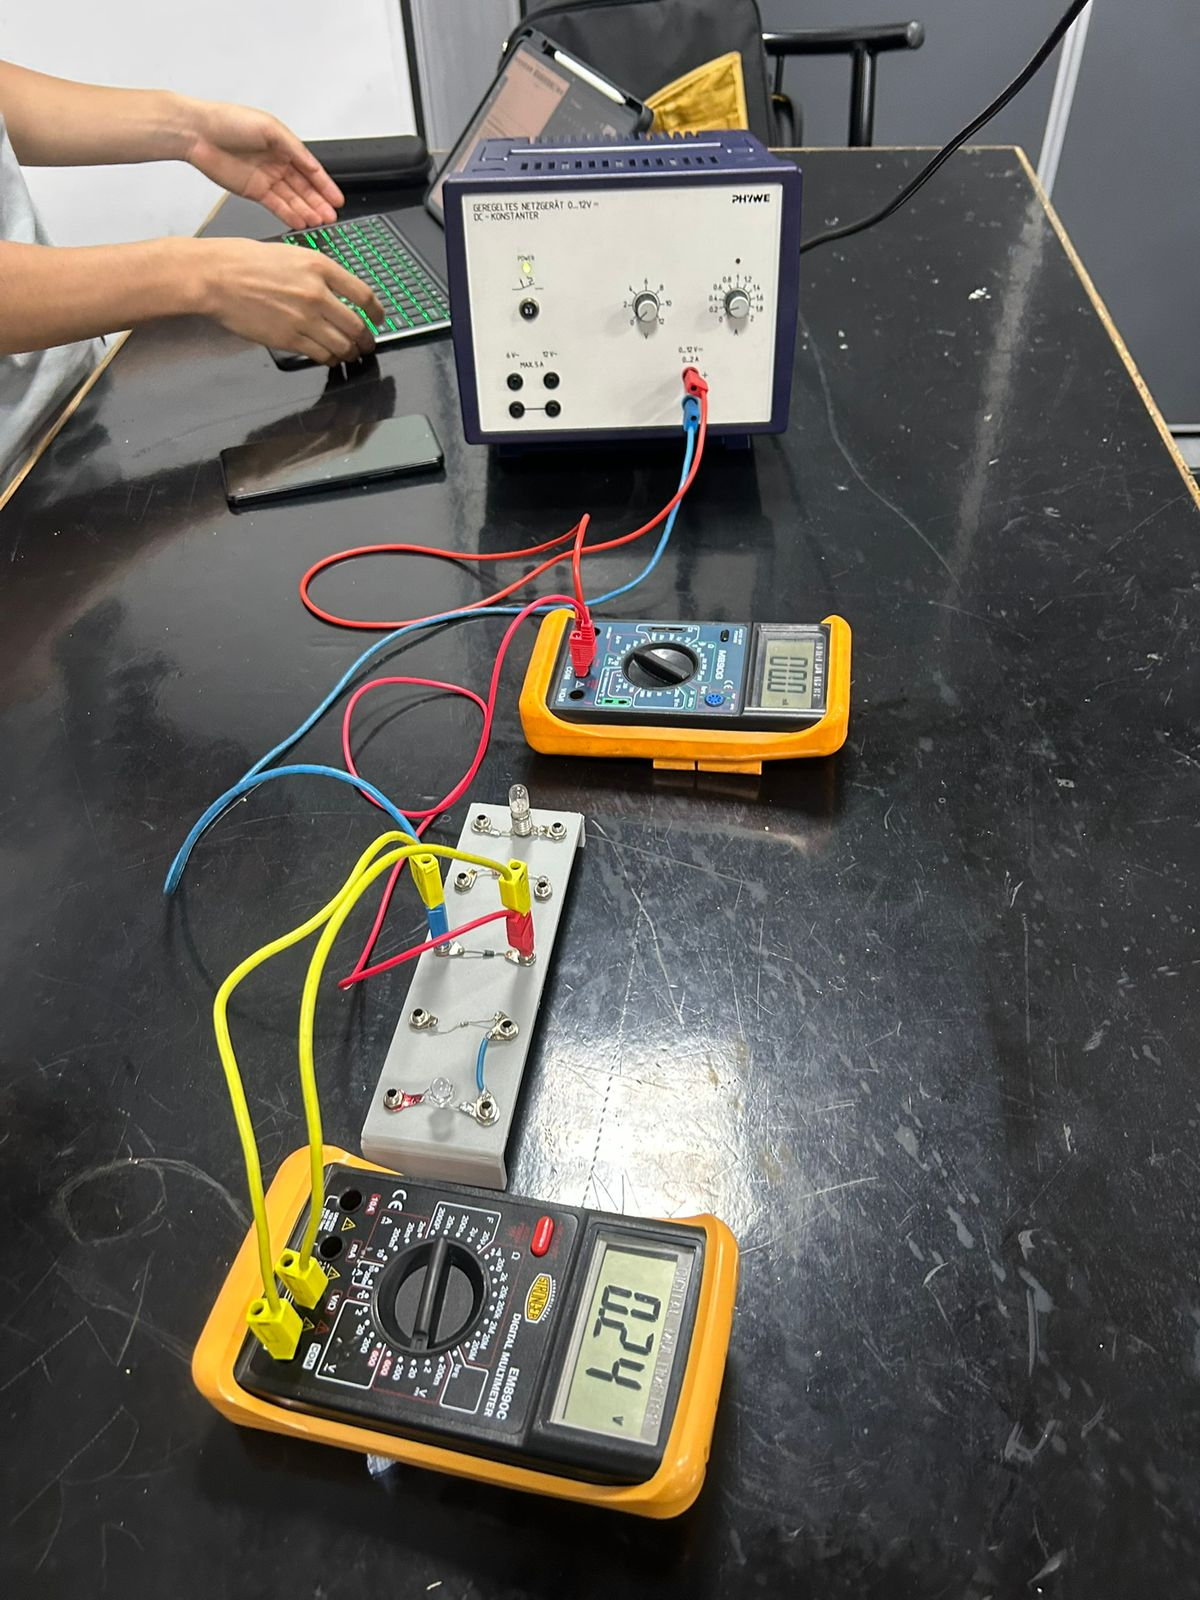
\includegraphics[width=0.8\textwidth]{foto_elementos.jpeg} 
    \caption{Disposición de los instrumentos de medición y componentes en el banco de trabajo, junto con la fuente de tensión.}
    \label{fig:fotos_laboratorio}
\end{figure}

\vspace{0.4cm}

\subsection{Circuitos de medición}
El montaje experimental se realizó siguiendo los esquemas de la Figura \ref{fig:circuitos_detallados}. Se optó por una configuración de medición donde el voltímetro mide directamente la tensión sobre el componente, asegurando que la resistencia interna del instrumento no afectara significativamente los resultados dada la magnitud de las corrientes medidas.

\vspace{0.3cm}

\begin{figure}[H]
    \centering
    % --- SUBFIGURA 1: RESISTOR ---
    \begin{subfigure}{0.48\textwidth}
        \centering
        \begin{circuitikz}[scale=0.8, transform shape]
            \draw (0,0) to[american voltage source, invert, l=$V_{f}$] (0,3)
            to[ammeter, l=$I$] (3,3)
            to[R, l=$R$, *-, v=$V_R$] (3,0)
            (3,3) -- (5,3)
            to[voltmeter, l=$V$] (5,0) -- (0,0);
        \end{circuitikz}
        \caption{Resistor de carbón ($\SI{220}{\ohm}$)}
        \label{fig:circ_resistor}
    \end{subfigure}
    \hfill
    % --- SUBFIGURA 2: LÁMPARA ---
    \begin{subfigure}{0.48\textwidth}
        \centering
        \begin{circuitikz}[scale=0.8, transform shape]
            \draw (0,0) to[american voltage source, invert, l=$V_{f}$] (0,3)
            to[ammeter, l=$I$] (3,3)
            to[lamp, l=L, *-, v=$V_L$] (3,0)
            (3,3) -- (5,3)
            to[voltmeter, l=$V$] (5,0) -- (0,0);
        \end{circuitikz}
        \caption{Lámpara de filamento}
        \label{fig:circ_lampara}
    \end{subfigure}

    \vspace{0.8cm}

    % --- SUBFIGURA 3: DIODO SILICIO ---
    \begin{subfigure}{0.48\textwidth}
        \centering
        \begin{circuitikz}[scale=0.8, transform shape]
            \draw (0,0) to[american voltage source, invert, l=$V_{f}$] (0,3)
            to[ammeter, l=$I$] (3,3)
            to[D, l=D, *-, v=$V_D$] (3,0)
            (3,3) -- (5,3)
            to[voltmeter, l=$V$] (5,0) -- (0,0);
        \end{circuitikz}
        \caption{Diodo de Silicio}
        \label{fig:circ_diodo}
    \end{subfigure}
    \hfill
    % --- SUBFIGURA 4: LED CON RESISTENCIA (Voltímetro solo en LED) ---
    \begin{subfigure}{0.48\textwidth}
        \centering
        \begin{circuitikz}[scale=0.8, transform shape]
            \draw (0,0) to[american voltage source, invert, l=$V_{f}$] (0,3)
            to[ammeter, l=$I$] (3,3)
            to[R, l=$R_p$] (3,1.5)                % Resistencia de protección hasta el punto medio
            to[led, l=LED, *-, v=$V_{LED}$] (3,0)
            
            % Conexión del voltímetro desde el nodo intermedio (3, 1.5)
            (3,1.5) -- (5,1.5) 
            to[voltmeter, l=$V$] (5,0) -- (0,0);
        \end{circuitikz}
        \caption{LED con resistencia de protección}
        \label{fig:circ_led}
    \end{subfigure}

    \caption{Esquemas eléctricos para el relevamiento de cada componente.}
    \label{fig:circuitos_detallados}
\end{figure}

\pagebreak